\section{Hydraulic modelling}
\label{HydraulicModel}

Water distribution networks are designed to deliver water to consumers in terms of sufficient pressure and appropriate chemical composition. Distribution systems as such are generally consisting of four main components: pipes, pumps, valves and reservoirs. The common property is that they are all two-terminal components, therefore they can be characterized by the dynamic relationship between the pressure drop across the two endpoints and the flow through the element \cite{Kallesoe2009}.  \eqref{onecomponent} shows the dual variables which describe one component. 

\begin{equation}
\label{onecomponent}
 \begin{bmatrix}
    \Delta P \\
    q
\end{bmatrix}
=
 \begin{bmatrix}
    P_{in} - P_{out} \\
    q
\end{bmatrix}
\end{equation}

 \begin{minipage}[t]{0.20\textwidth}
Where\\
\hspace*{8mm} $\Delta p$ \\
and \hspace*{0.7mm} $q$ 
\end{minipage}
\begin{minipage}[t]{0.68\textwidth}
\vspace*{2mm}
is the pressure drop across the two endpoints,\\
is the flow through the element.
\end{minipage}
\begin{minipage}[t]{0.10\textwidth}
\vspace*{2mm}
\textcolor{White}{te}$\unit{Pa}$\\
\textcolor{White}{te}$\unit{\frac{m^{3}}{s}}$ 
\end{minipage}

In the following chapter, the hydraulic model of the system is derived by control volume approach \cite{Hunt_Fluidmechanics}. The relationship between the two variables is introduced for each component in the hydraulic network.

\subsection{Pipe model} 
\label{PipeModel}
Pipes are important components of water distribution systems since they are used for carrying pressurized water. A detailed model of the pipes has to be derived in order to understand the relationship of pressure and flow for each pipe component.  
%
The dynamic model of a pipe can be originated from Newton's second law. \eqref{NewtonLaw} describes the proportionality between the rate of change regarding the momentum of the water and the force acting on it.

\begin{equation}
  \frac{d}{dt} M = \sum_i F_i
  \label{NewtonLaw}
\end{equation} 

\begin{minipage}[t]{0.20\textwidth}
Where\\
\hspace*{8mm} $M$ \\
and \hspace*{0.7mm}  $F_i$ 
\end{minipage}
\begin{minipage}[t]{0.68\textwidth}
\vspace*{2mm}
is the linear momentum of the water flow,\\
is the set of forces acting on the water.
\end{minipage}
\begin{minipage}[t]{0.10\textwidth}
\vspace*{2mm}
\textcolor{White}{te}$\unit{\frac{kgm}{s^2}}$\\
\textcolor{White}{te}$\unit{N}$
\end{minipage}

The dynamic model of a pipe component is derived under the assumption that the flow of the fluid is uniformly distributed along the cross sectional area of the pipe. In other words, all pipes in the system are filled up fully with water all the time. Thus, the density of water and the volume of the fluid is constant in time, as the mass of the water.
\\
Rewriting \eqref{NewtonLaw}, due to the above-mentioned asumptions, the mass of the water can be taken out in front of the derivative.

\begin{equation}
  \frac{d}{dt} M = {\frac{d(m_w v)}{dt}} = m_w \frac{dv}{dt} = \sum_i F_i
\end{equation} 

\begin{minipage}[t]{0.16\textwidth}
Where\\
\hspace*{8mm} $m_w$ \\
and \hspace*{0.7mm} $v$ 
\end{minipage}
\begin{minipage}[t]{0.72\textwidth}
\vspace*{2mm}
is the mass of the water,\\
is the value of the velocity of the water at each point of the pipe.
\end{minipage}
\begin{minipage}[t]{0.10\textwidth}
\vspace*{2mm}
\textcolor{White}{te}$\unit{kg}$\\
\textcolor{White}{te}$\unit{\frac{m}{s}}$
\end{minipage}

The sum of the forces acting on the control volume can be seen as input forces, acting on the inlet of the pipe and output forces acting on the outlet. Furthermore, resistance forces and the effect of gravitational force is present.  
These forces are expressed in terms of pressure in order to obtain the model of the pressure drop in the pipes. In \figref{fig:pipe_freebody}, all forces acting on a pipe segment are shown:
%
%tikz of the pipe freebody diagram
\begin{figure}[H]
\centering
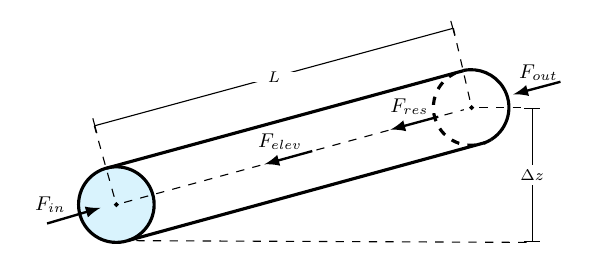
\begin{tikzpicture} [scale=0.8,transform shape]

  \draw[|-|] (4.1,-2.6) --
        node[fill=white,font=\scriptsize,inner ysep=2pt,inner
                xsep=20]{$\Delta z$}(4.1,-0.46) node (v5) {};
                
 \draw[|-|] (2.85,0.8) --
        node[fill=white,font=\scriptsize,inner ysep=0pt,inner
                xsep=20]{$L$}(-2.85,-0.75)  {};
                
 \fill[cyan!15] (-2.5,-2) circle (0.6cm);
\draw [line width=0.4mm, black ] (-2.5,-2) node (v2) {} circle (0.6cm);


\draw [line width=0.4mm, black ] (-2.65,-1.42) node (v6) {} -- (3.01,0.126);

\draw [line width=0.4mm, black] (3.45,-0.967) node (v1) {} arc (-58:102:0.6);
\draw [line width=0.4mm, black, dashed] (3.45,-0.967) node (v1) {} arc (302:115:0.6); %% Dashed circle


\draw[black,fill=black] (-2.5,-2) node (v7) {} circle (.2ex);

\draw [line width=0.4mm, black ] (-2.32,-2.572) node (v3) {} -- (3.36,-1.014); %% Lower line
\draw [black,fill=black] (3.14,-0.46) node (v4) {} circle (.2ex); 	% Upper dot

\draw [dashed=on 2pt off 3pt on 4pt off 4pt](v3) -- (4.1,-2.6) ;
\draw [dashed=on 2pt off 3pt on 4pt off 4pt](v4) -- (v5);


\draw [dashed](v7) -- (-2.85,-0.75);
\draw [dashed](v4) -- (2.85,0.8);
\draw [dashed](v7) -- (v4);


\draw [line width=0.3mm, black ] [-latex](-3.6,-2.3) -- (-2.75,-2.05);

\draw [line width=0.3mm, black ] [-latex](4.55,-0.05) -- (3.8,-0.25);

\draw [line width=0.3mm, black ] [-latex](2.61,-0.605) -- (1.85,-0.8105);

\draw [line width=0.3mm, black ] [-latex](0.61,-1.15) -- (-0.15,-1.36);

\node at (-3.55,-2) {\small{$F_{in}$}};
\node at (4.2,0.1) {\small{$F_{out}$}};
\node at (2.15,-0.45) {\small{$F_{res}$}};
\node at (0.1,-1) {\small{$F_{elev}$}};
\end{tikzpicture}% 
\caption{Free-body diagram describing the forces acting on a segment of a pipe.}
\label{fig:pipe_freebody}
\end{figure}
%
The pipe is assumed to have a cylindrical structure. Furthermore, the cross section of the pipe, $A(x)$, is constant for every $x \in [0,L]$, where $L$ is the length of the pipe:

\begin{equation}
  A_{in} = A_{out} = \frac{1}{4}\pi D^{2}
\end{equation}

 \begin{minipage}[t]{0.20\textwidth}
Where\\
\hspace*{8mm} $A$ \\
and \hspace*{0.7mm} $D$
\end{minipage}
\begin{minipage}[t]{0.68\textwidth}
\vspace*{2mm}
is the cross sectional area of a pipe,\\
is the diameter of the pipe.
\end{minipage}
\begin{minipage}[t]{0.10\textwidth}
\vspace*{2mm}
\textcolor{White}{te}$\unit{m^{2}}$\\
\textcolor{White}{te}$\unit{m}$
\end{minipage}

Water flow, $q$, can be expressed in terms of velocity, $v$, and cross sectional 
area, $A$, resulting in:\\
%Continuity law in fluid mechanics is applied to analyze the flow in the pipe\cite{Hunt_Fluidmechanics}. A steady and uniform mass flow is assumed in the pipe. Hence, the water flow can be described as: 
\begin{equation}
  q=A \cdot v
	\label{EquationOfContinuity}
\end{equation}

 In \eqref{LinearMomentum} the forces acting on the pipe are included. The difference between $F_{in}$ and $F_{out}$ defines the ideal pressure drop between the two endpoints, without taking into account the resistance forces $F_{res}$ and the gravitational force effect due to change in elevation $F_{elev}$.

\begin{equation}
  m_w \frac{dv}{dt} = F_{in} - F_{out} - F_{res} - F_{elev} \\
  \label{LinearMomentum}
\end{equation}

In order to obtain an equation consisting of only pressure variables, the relationship between forces and pressures is used.


 \begin{equation}
    A L \rho \frac{dv}{dt} = A (\textit{p}_{in} - \textit{p}_{out}) - F_{res} - F_{elev} \\
\end{equation}

\begin{minipage}[t]{0.20\textwidth}
Where\\
\hspace*{8mm} $m_w$ \\
\hspace*{8mm} $L$ \\
\hspace*{8mm} $\rho$\\
and \hspace*{0.7mm} $p$ 
\end{minipage}
\begin{minipage}[t]{0.68\textwidth}
\vspace*{2mm}
is the mass of the water,\\
is the length of a pipe,\\
is the water density,\\
is the pressure.
\end{minipage}
\begin{minipage}[t]{0.10\textwidth}
\vspace*{2mm}
\textcolor{White}{te}$\unit{kg}$\\
\textcolor{White}{te}$\unit{m}$\\
\textcolor{White}{te}$\unit{\frac{kg}{m^{3}}}$
\textcolor{White}{te}$\unit{Pa}$\\
\end{minipage}
%
Rewriting the velocity in terms of volumetric water flow and cross sectional 
area according to \eqref{EquationOfContinuity}:

\begin{equation}
    A L \rho \frac{d}{dt} \frac{q}{A} = A (\textit{p}_{in} -  \textit{p}_{out}) - F_{res} - F_{elev}\\
\end{equation}

By dividing the equation with the cross sectional area it can be seen that the equation is dependent on the pressure difference between two endpoints.
%Reducing the cross sectional area to obtain an expression for the pressure: 

\begin{equation}
    \frac{L \rho}{A} \frac{dq}{dt} =p_{in} - p_{out} - \frac{ F_{res} - F_{elev}}{A} \\
\end{equation}

Thus the desired pressure drop between two endpoint is obtained. The differential equation in \eqref{PressureDrop}, describes the change in flow as a function of the pressure drops in the system.

\begin{equation}
    \frac{L \rho}{A} \frac{dq}{dt} =\Delta p - \frac{ F_{res} - F_{elev}}{A} \\
    \label{PressureDrop}
\end{equation}

In \eqref{PressureDrop}, the term $F_{res}$ is the resistance force acting on the 
pipe, which consists of two parts: surface resistance($h_{f}$) and the form resistance($h_{m}$) due to the fittings. % $F_{elev}$ is the force of gravity due to change in elevation, $\Delta z$.

\textbf{Surface resistance (\texorpdfstring{$h_f$}{})} \\
The flow of liquid through pipes is affected by resistance from 
the turbulence occurring along the internal walls of the pipe, caused by the roughness of the pipe surface. The surface resistance is given by the Darcy-Weisbach equation \cite{Design_Water}.

%\todo{Should we find another formulation then "pressure given in head" - Kind of wierd to to have pressure given as 'm'}

\begin{equation}
  h_f = \frac{fLv^2}{2gD}
  \label{Darcy}
\end{equation}

 \begin{minipage}[t]{0.20\textwidth}
Where\\
\hspace*{8mm} $f$ \\
\hspace*{8mm} $h_f$ \\
and\hspace*{0.7mm} $g$ 
\end{minipage}
\begin{minipage}[t]{0.68\textwidth}
\vspace*{2mm}
is the Moody friction factor,\\ 
is the pressure given in head,\\   
is the gravitational constant.
\end{minipage}
\begin{minipage}[t]{0.10\textwidth}
\vspace*{2mm}
\textcolor{White}{te}$\unit{\cdot}$\\
\textcolor{White}{te}$\unit{m}$\\
\textcolor{White}{te}$\unit{\frac{m}{s^2}}$
\end{minipage}

\eqref{Darcy} is valid under the assumption that $v>0$. %, therefore it is not dependant on $|v|v$ but on $v^2$. \\
 Assuming that the flow is not unidirectional and substituting the velocity by the volumetric flow and pipe area:

\begin{equation}
  h_f = \frac{8fL}{\pi^{2}gD^5} |q| q
  \label{DarcyWeisbach}
\end{equation} 
 
 The unknown parameter in \eqref{DarcyWeisbach} is the Moody friction factor 
 which is non-dimensional and is a function of the Reynold's number, $Re$. This friction factor depends on whether the flow is laminar, transient or turbulent, and the roughness of the pipe \cite{Intro_Fluid}.  
 
The Reynold's number can be used to determine the regime of the flow \cite{Intro_Fluid}. When $Re<2300$ as laminar, if $2300<Re<4000$ as transient and if
$Re>4000$ as turbulent. 

\begin{equation}
   Re = \frac{vD}{\nu}
   \label{Reynolds}
 \end{equation}
 
  \begin{minipage}[t]{0.20\textwidth}
Where\\
\hspace*{8mm} $\nu$ 
\end{minipage}
\begin{minipage}[t]{0.68\textwidth}
\vspace*{2mm}
is the kinematic viscosity.

\end{minipage}
\begin{minipage}[t]{0.10\textwidth}
\vspace*{2mm}
\textcolor{White}{te}$\unit{\frac{kg}{ms}}$
\end{minipage}

The kinematic viscosity according to \cite{Design_Water} is given by :

\begin{equation}
  \nu = 1.792 \cdot 10^{-6} \Bigg[1+{\bigg(\frac{T}{25}\bigg)}^{1.165} \Bigg]^{-1}
\end{equation}

  \begin{minipage}[t]{0.20\textwidth}
Where\\
\hspace*{8mm} $T$ 
\end{minipage}
\begin{minipage}[t]{0.68\textwidth}
\vspace*{2mm}
is the water temperature.
 \end{minipage}
\begin{minipage}[t]{0.10\textwidth}
\vspace*{2mm}
\textcolor{White}{te}$\unit{^{\circ} C}$
\end{minipage}

In order to estimate the range of Reynolds numbers in a common water 
distribution, typical values for the temperature, velocity and the radius of 
the pipes are considered \cite{Urban_Design}. 

% \begin{itemize}
%   \item $v = 0.5 - 1.5  \quad \frac{m}{s}$
%   \item $D = 50 - 1500\quad mm$
%   \item $T = 10 - 20 \quad ^{\circ} C$
% \end{itemize}

\begin{itemize}
  \item $ v \in [0.5,1.5] \unit{\frac{m}{s}}$
  \item $ D \in [50,1500]\unit{mm}$
  \item $T \in [10,20] \unit{^{\circ} C} $
\end{itemize}

These values result in a Reynold's number between 19000 and 225000, which is considered as turbulent fluid flow through the pipes. For turbulent flow, the 
Moody friction factor is given by \cite{Design_Water}: 

\begin{equation}
  f = 1.325 \bigg(ln\bigg(\frac{\epsilon}{3.7 D}+\frac{5.74}{Re^{0.9}}\bigg)\bigg)^{-2}
  \label{turbulent}
\end{equation}

\begin{minipage}[t]{0.20\textwidth}
Where\\
\hspace*{8mm} $\epsilon$ 
\end{minipage}
\begin{minipage}[t]{0.68\textwidth}
\vspace*{2mm}
is the average roughness of the wall inside the pipe.
 \end{minipage}
\begin{minipage}[t]{0.10\textwidth}
\vspace*{2mm}
\textcolor{White}{te}$\unit{m}$
\end{minipage}

%
\textbf{Form resistance (\texorpdfstring{$h_m$}{})} 
\label{FormResistance}

Form resistance losses are present at any time the flow changes direction, due to elbows, bends, enlargers and reducers. It is a particular frictional resistance due to the 
fittings of a pipe. Form loss can be expressed as: 

\begin{equation}
  h_m = k_f \frac{v^2}{2g}
\end{equation}


Applying the definition of volumetric flow:

\begin{equation}
   h_m = k_f \frac{8}{\pi^2gD^4}  |q| q
\label{Formloss}
\end{equation}

 \begin{minipage}[t]{0.20\textwidth}
Where\\
\hspace*{8mm} $k_f$ 
\end{minipage}
\begin{minipage}[t]{0.68\textwidth}
\vspace*{2mm}
is the form-loss coefficient.  
 \end{minipage}
\begin{minipage}[t]{0.10\textwidth}
\vspace*{2mm}
\textcolor{White}{te}$\unit{\cdot}$
\end{minipage}

The form-loss coefficient can be split into different losses depending on the 
fitting of the pipes. 
\\
Pipe bends are principally determined by the 
bend angle $\alpha$ and bend radius $r$. This is given by the following 
expression \cite{Design_Water}: 

\begin{equation}
  k_f = \bigg[0.0733 + 0.923 \bigg(\frac{D}{r}\bigg)^{3.5}\bigg]\alpha^{0.5}
  \label{kfriction}
\end{equation}

Pipe elbows are also used to change the direction of the flow, however providing 
sharp turns in pipelines. The coefficient for the losses in elbows is determined by the angle of an elbow $\alpha$ and is given by:

\begin{equation}
  k_f = 0.442\alpha^{2.17}
\end{equation}

\textbf{Complete pipe model}
\label{CompletePipe}    % If we remove this subsection we have to change the 
% reference to it in the Parameter Estimation subsection

In \eqref{DarcyWeisbach} and \eqref{Formloss}, the head loss of the friction losses are determined. These terms are introduced in \eqref{PressureDrop} in terms of pressure. The friction factors are multiplied by the water density and gravity. Nevertheless, the head loss due to elevation has to be added in the model, yielding the final expression:

\begin{equation}
   \frac{L \rho}{A} \frac{dq}{dt} =\Delta p - h_f \rho g - h_m \rho g - \Delta z_h \rho g
\end{equation}
 \begin{minipage}[t]{0.20\textwidth}
Where\\
\hspace*{8mm} $\Delta z_h$ \\
\end{minipage}
\begin{minipage}[t]{0.68\textwidth}
\vspace*{2mm}
the head loss due to elevation.
\end{minipage}
\begin{minipage}[t]{0.10\textwidth}
\vspace*{2mm}
\textcolor{White}{te}$\unit{m}$
\end{minipage}

Substituting the terms $h_f$ and $h_m$ with their respective values:

\begin{equation}
\label{FinalPipeModel}
   \frac{L \rho}{A} \frac{dq}{dt} =\Delta p - \frac{8fL}{\pi^{2}gD^5} \rho g  |q| q - k_f \frac{8}{\pi^2gD^4} \rho g |q| q - \Delta z_h \rho g 
\end{equation}

\eqref{FinalPipeModel} describes the rate of flow in terms of pressure losses due to pressure change, frictions and elevation. Introducing a function for the pressure drop due to friction in the pipes, the following expression can be written up for the $k^{th}$component:

\begin{equation}
\label{FinalPipeModelCompact}
   J_k \dot{q_k} = \Delta p_k - \lambda_k(q_k) - \zeta_k 
\end{equation}

 \begin{minipage}[t]{0.20\textwidth}
Where\\
\hspace*{8mm} $J_k$ \\
\hspace*{8mm} $\lambda_k(q_k)$ \\
and \hspace*{0.7mm} $\zeta_k$ 
\end{minipage}
\begin{minipage}[t]{0.68\textwidth}
\vspace*{2mm}
is an analogous parameter as inertia for the water,\\ 
is the friction as a function of flow,\\
is the pressure drop due to elevation.
\end{minipage}

As can be seen in \eqref{FinalPipeModelCompact}, the flow dynamics of the $k^{th}$ pipe is described by $J_k$, which is an analogous parameter as inertia in mechanical systems. $\bm{J}$ is a diagonal matrix with zeros for the diagonal elements not related to pipe components, $\pmb{J} = diag(J_k)$.

It is assumed, prior to the tests carried out on the system, that the presence of the WT in the system has a slow effect on the flow due to its slow integration behavior. This means that the WT assumed to have a relatively big time constant compared to the pipes. Due to this consideration, a fair assumption is that the parameter $J_k$ does not influence the flow in the system significantly and therefore it could be neglected. However, the parameter is kept, until this assumption is verified by tests. The complete model of a pipe yields: 
  
\begin{equation}
\label{FinalPipeModelSimplified}
  \Delta p_k  =   \lambda_k(q_k) + J_k \dot{q_k} + \zeta_k 
\end{equation}


